\documentclass[ma3408.tex]{subfiles}
\begin{document}
\chapter{Fiber bundles}
\section{Locally trivial bundles}
We begin with what we will call a locally trivially bundle.\footnote{Confusingly, some books will also call this a fiber bundle. We will see why later.}
\begin{Def}
A map $\pi \colon E\to B$ is a locally trivial bundle with fiber $F$ if the following conditions hold:
\begin{enumerate}
	\item Each point $b \in B$ has a neighbourhood $U$ such that $\pi^{-1}(U_b) \xrightarrow{h_b} U_b \times F$.
	\item The following diagram commutes
	% https://q.uiver.app/?q=WzAsMyxbMCwwLCJcXHBpXnstMX0oVV9iKSJdLFsyLDAsIlVfYiBcXHRpbWVzIFxccGleey0xfShiKSJdLFsxLDEsIlVfYiJdLFswLDEsImhfYiJdLFswLDIsIlxccGkiLDJdLFsxLDIsIlxcdGV4dHtwcn1fMSJdXQ==
\[\begin{tikzcd}[ampersand replacement=\&]
	{\pi^{-1}(U_b)} \&\& {U_b \times F} \\
	\& {U_b}
	\arrow["{h_b}", from=1-1, to=1-3]
	\arrow["\pi"', from=1-1, to=2-2]
	\arrow["{\text{pr}_1}", from=1-3, to=2-2]
\end{tikzcd}\]
\end{enumerate}
The maps $h_b$ are called the \emph{local trivializations} of the bundle.
\end{Def}
\begin{Exa}
Let $E = B \times F$ and $\pi \colon E  = B \times F \to B$ the projection map. This is called the trivial bundle. 
\end{Exa}
\begin{Exa}
If $F$ is discrete, then a locally trivial bundle with fiber $F$ is a covering map. 
\end{Exa}
\begin{Exa}\label{exa:mobius}
The M{\"o}bius band is a locally trivial bundle with fiber $S^1$, see \Cref{fig:mob}. 
\begin{figure}[h!] \centering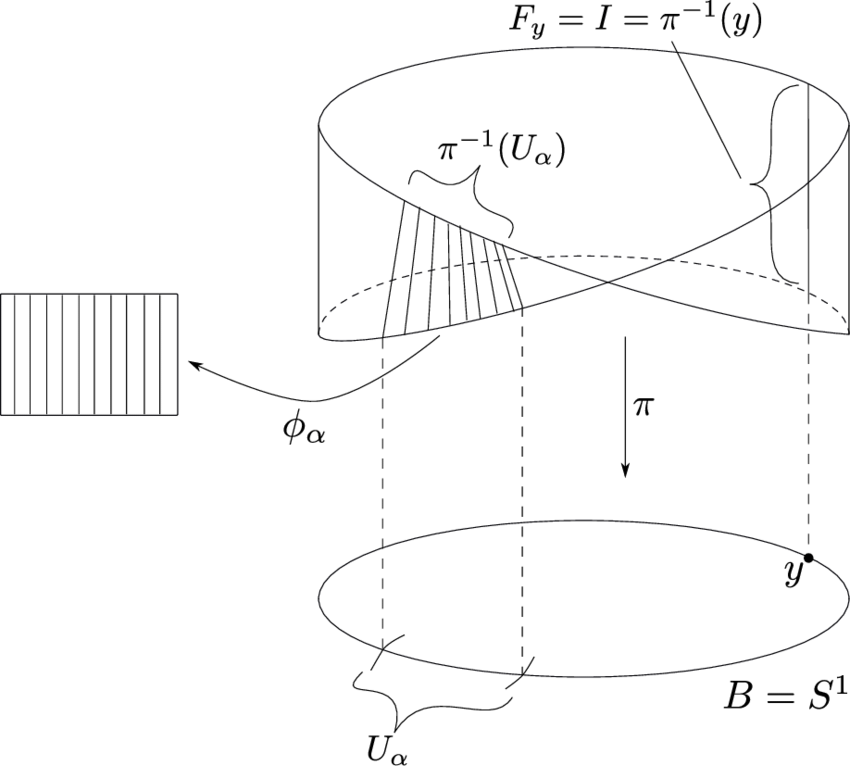
\includegraphics[scale = 0.25]{mob.png}\caption{The M{\"o}bius band}\label{fig:mob}\end{figure}
We will return to this example in due course. 
\end{Exa}
\begin{Rem}
We can write a locally trivial bundle as $F \to E \to B$, which is reminiscent of the notation for a fibration. In fact, fiber bundles over paracompact base spaces are always fibrations.\footnote{A space is paracompact if every open cover has an open refinement that is locally finite. } More generally, any locally trivial bundle is a Serre fibration. 
\end{Rem}
\begin{Rem}
Let us unwind the definition of a locally trivial bundle a little more. Let $\pi \colon E \to B$ be a locally trivial bundle with fiber $F$. From the definition we can cover $B$ by a family of open sets $\{ U_{\alpha} \}$ such that each inverse image $\pi^{-1}(U_{\alpha})$ is fiberwise homeomorphic to $U_{\alpha} \times F$ . This gives a system of homeomorphisms
\[
\phi_{\alpha} \colon U_{\alpha} \times F \to \pi^{-1}(U_{\alpha}). 
\]
Observe that if $V \subseteq U_{\alpha}$ then the restriction of $\phi_{\alpha}$ to $V \times F$ gives the homeomorphism with $\pi^{-1}(V)$. Hence on $U_{\alpha} \cap U_{\beta}$ there are two fiberwise homeomorphisms
\[
\begin{split}
\phi_{\alpha} &\colon (U_{\alpha} \cap U_{\beta})\times F \to \pi^{-1}(U_{\alpha} \cap U_{\beta})\\
\phi_{\beta} &\colon (U_{\alpha} \cap U_{\beta})\times F \to \pi^{-1}(U_{\alpha} \cap U_{\beta})
\end{split}
\]
Consider the following commutative diagram
% https://q.uiver.app/?q=WzAsNCxbMCwwLCIoVV97XFxhbHBoYX0gXFxjYXAgVV97XFxiZXRhfSkgXFx0aW1lcyBGIl0sWzEsMCwiXFxwaV57LTF9KFVfe1xcYWxwaGF9IFxcY2FwIFVfe1xcYmV0YX0pIl0sWzIsMCwiKFVfe1xcYWxwaGF9IFxcY2FwIFVfe1xcYmV0YX0pIFxcdGltZXMgRiJdLFsxLDEsIlVfe1xcYWxwaGF9IFxcY2FwIFVfe1xcYmV0YX0iXSxbMCwxLCJcXHBoaV97XFxhbHBoYX0iXSxbMSwyLCJcXHBoaV97XFxiZXRhfV57LTF9Il0sWzEsM10sWzAsM10sWzIsM11d
\[\begin{tikzcd}[ampersand replacement=\&]
	{(U_{\alpha} \cap U_{\beta}) \times F} \& {\pi^{-1}(U_{\alpha} \cap U_{\beta})} \& {(U_{\alpha} \cap U_{\beta}) \times F} \\
	\& {U_{\alpha} \cap U_{\beta}}
	\arrow["{\phi_{\alpha}}", "\cong"', from=1-1, to=1-2]
	\arrow["{\phi_{\beta}^{-1}}", "\cong"',from=1-2, to=1-3]
	\arrow[from=1-2, to=2-2]
	\arrow[from=1-1, to=2-2]
	\arrow[from=1-3, to=2-2]
\end{tikzcd}\]
Let $\phi_{\alpha\beta}$ denote the top composite $\phi_{\beta}^{-1}\phi_{\alpha}$. Then the locally trivially bundle is completed determined by the base $B$, the fiber $F$, the covering $U_{\alpha}$ and the homeomorphisms $U_{\alpha\beta}$. Roughly speaking, $E$ should be thought of as the cartesian product of the $U_{\alpha} \times F$ with some identifications by the $\phi_{\alpha\beta}$. 
\end{Rem}
\begin{Def}
The open sets $U_{\alpha}$ are called \emph{charts}, the family $U_{\alpha}$ the \emph{atlas of charts}, the homeomorphisms $\phi_{\alpha}$ are called the \emph{coordinate homeomorphisms} and the $\phi_{\alpha\beta}$ are called the \emph{transition functions.}
\end{Def}
\begin{Rem}
In order for homeomorphisms $\phi_{\alpha\beta}$ to be the transition functions of a locally trivial bundle, they must satisfy, $\phi_{\alpha\beta} = \phi_{\beta}^{-1}\phi_{\alpha}$. For example,
\[
\phi_{\alpha\alpha} = \text{id} 
\]
and
\[
 \phi_{\gamma\alpha}\phi_{\beta\gamma}\psi_{\alpha\beta} = \text{id}
\]
on any triple $(U_{\alpha} \cap U_{\beta} \cap U_{\gamma}) \cap F$. Taking $\gamma = \alpha$ we get
\[
\phi_{\alpha\beta}\phi_{\beta\alpha} = \text{id}.
\]
In fact, these conditions suffices to reconstruct the locally trivial bundle for the base, the fiber, atlas and homeomorphisms. Indeed, set $E = E'/\sim$ where
\[
E' = \bigcup_{\alpha} (U_{\alpha} \times F)
\]
and for $(x,f) \in U_{\alpha} \times F$ and $(y,g) \in U_{\beta} \times F$ we have $(x,f) \sim (y,g) \iff x = y \in (U_{\alpha} \cap U_{\beta})$ and $(y,g) = \phi_{\alpha\beta}(x,f)$. It is a rather tedious exercise to show that this determines a locally trivial bundle. 
\end{Rem}
\begin{Def}
Two locally trivial bundles $\pi \colon E \to B$ and $\pi' \colon E' \to B'$ are isomorphic if there is a homeomorphism $\psi \colon E \to E'$ such that the diagram
% https://q.uiver.app/?q=WzAsMyxbMCwwLCJFIl0sWzIsMCwiRSciXSxbMSwxLCJGIl0sWzAsMSwiXFxwc2kiXSxbMCwyLCJcXHBpIiwyXSxbMSwyLCJcXHBpJyJdXQ==
\[\begin{tikzcd}[ampersand replacement=\&]
	E \&\& {E'} \\
	\& B
	\arrow["\psi", from=1-1, to=1-3]
	\arrow["\pi"', from=1-1, to=2-2]
	\arrow["{\pi'}", from=1-3, to=2-2]
\end{tikzcd}\]
commutes. (Note that this implies that there is a homeomorphism $F \to F'$ between the fibers as well).
\end{Def}
\begin{Thm}
Two systems of transition functors $\phi_{\beta\alpha}$ and $\phi_{\beta\alpha}'$ define isomorphic locally trivial bundles iff there exists fiber preserving homeomorphisms
\[
h_{\alpha} \colon U_{\alpha} \times F \to U_{\alpha} \times F
\]
such that $\phi_{\beta\alpha}= h_{\beta}^{-1}\phi'_{\beta\alpha}h_{\alpha}$. 
\end{Thm}
\begin{proof}
First, we suppose that the two bundles are isomorphic, so in particular there is a homeomorphism $\psi \colon E \to E'$. We let 
\[h_{\alpha} \coloneqq \phi_{\alpha}^{'-1}\psi^{-1}\phi_{\alpha}\colon U_{\alpha} \times F \to U_{\alpha} \times F. 
\]
Then we have
\[
\begin{split}
h_{\beta}^{-1}\phi'_{\beta\alpha}h_{\alpha} &= \phi_{\beta}^{-1}\psi^{-1}\phi'_{\beta}\phi'_{\beta\alpha}\phi_{\alpha}^{-1}\psi^{-1}\phi_{\alpha}\\
&=\phi_{\beta}^{-1}\psi^{-1}\phi_{\beta'}\phi_{\beta}^{'-1}\phi'_{\alpha}\phi_{\alpha}^{-1}\psi^{-1}\phi_{\alpha} = \phi_{\beta\alpha}.
\end{split}
\]
Conversely, if the relations hold, then we set $\psi = \phi_{\alpha}h_{\alpha}^{-1}\phi^{'-1}_{\alpha}$. A similar argument then shows that $\phi_{\beta}h_{\beta}^{-1}\phi^{'-1}_{\beta} = \phi_{\alpha}h_{\alpha}^{-1}\phi{'-1}_{\alpha}$. 
\end{proof}
\begin{Rem}\label{rem:not_a_trivial_bundle}
If $\pi$ is (isomorphic to) a trivial bundle, then all transition functions can be chosen to be the identity. One can use the previous theorem to show that a bundle is not isomorphic to a trivial bundle. 
\end{Rem}
\begin{Exa}\label{exa:mobius2}
After this discussion, let us return to the example of the M{\"o}bius bundle (\Cref{exa:mobius}). One can think of this as the space
\[
E = \{(x,y) \colon 0 \le x \le 1, 0 \le y \le 1 \}/\sim
\]
where we identify $(0,y)$ and $(1,1-y)$ for each $y \in [0,1]$. The projection maps $E$ to $I_x =\{ 0 \le x \le 1\}$ with the endpoints identified, that is, onto the circle. To see that this is a bundle we use the atlas
\[
U_{\alpha} = \{ 0 \le x \le 1 \}, \text{ and } U_{\beta} = \{ 0 \le x < 1/2\} \cup \{ 1/2 < x \le 1 \}. 
\]
We define
\[
\phi_{\alpha} \colon U_{\alpha} \times I_y \to E, \quad \phi_{\alpha}(x,y) = (x,y), 
\]
and
\[
\phi_{\beta} \colon U_{\beta} \times I_y \to E
\]
by
\[
\phi_{\beta} = \begin{cases}(x,y) & \text{for } 0 \le x \le /1/2, \\ (x,1-y) & \text{for } 1/2 < x \le 1.\end{cases}
\]
The intersection of these two charts is the union $(0,1/2) \cup (1/2,1)$, and the transition functions have the form
\[
\phi_{\beta\alpha} = (x,y) \text{ for } 0 < x < 1/2
\]
and 
\[
\phi_{\beta\alpha} = (x,1-y) \text{ for } 1/2 < x < 1.
\]
One can check from \Cref{rem:not_a_trivial_bundle} that the M{\"o}bius bundle is not isomorphic to a trivial bundle. 
\end{Exa}
We now give some more examples which will be useful in our study of characteristic classes. 
\begin{Def}
For $n<k$ the $n$-th Stiefel manifold associated to $\bbR^k$ is defined as
\[
V_n(\bbR^k) = \{ n-\text{frames in } \bbR^k \}
\]
where an $n$-frame in $\bbR^k$ is a tuple $\{v_1,\ldots,v_n\}$	of orthonormal vectors in $\bbR^k$, i.e., $v_1,\ldots,v_n$ are pairwise orthonormal, $\langle v_i,v_j \rangle = \delta_{ij}$. We given $V_n(\bbR^k)$ the subspace topology induced by thinking of it as a subspace of $S^{k-1} \times \ldots S^{k-1}$ ($n$-copies of $S^{k-1}$). 
\end{Def}
\begin{Exa}
A 1-frame is nothing but a unit vector, so the Stiefel manifold $V_1(\bbR^k)$ is the unit sphere in $\bbR^k$, i.e., $V_1(\bbR^k) \cong S^{k-1}$. On the other hand, an $n$-frame is an ordered basis, so $V_n(\bbR^n) \cong O(n)$. 
\end{Exa}
\begin{Def}
The $n$-th Grassmannian associated to $\bbR^k$ is defined as 
\[
G_n(\bbR^k) = \{ n-\text{dimensional vector subspaces in } \bbR^k \}
\]
There is a map $p \colon V_n(\bbR^k) \to G_n(\bbR^k)$ sending $\{ v_1,\ldots,v_n\}$ to the span, which is surjective by Gram--Schmidt, and we given $G_n(\bbR^k)$ the quotient topology. 
\end{Def}
\begin{Exa}
We have $G_1(\bbR^k)$ is the space of lines through the origin in $k$-space, so $G_1(\bbR^k) \simeq \bbR P^{k-1}$.
\end{Exa}
\begin{Lem}
	For $k>n$ the quotient map $p \colon V_n(\bbR^k) \to G_n(\bbR^k)$ is a locally trivial bundle with fiber $V_n(\bbR^n) \cong O(n)$, i.e., we have a locally trivial bundle
	\begin{equation}\label{eq:fiber-bundle-vn-gn}
	O(n) \to V_n(\bbR^k) \xrightarrow{p} G_n(\bbR^k). 
	\end{equation}
	Similarly, for $m <n \le k$ there are locally trivial bundles 
		\begin{equation}\label{eq:fiber-bundle-vn-vm}
	V_{n-m}(\bbR^k) \to V_n(\bbR^k) \xrightarrow{p} V_m(\bbR^k). 
	\end{equation}
	where the map $p$ takes $\{ v_1,\ldots,v_n\}$ to $\{ v_1,\ldots,v_m \}$. Taking $k =n$ we get a locally trivial bundle
			\begin{equation}\label{eq:fiber-bundle-on-vm}
	O(n-m) \to O(n) \xrightarrow{p} V_m(\bbR^n). 
	\end{equation}
\end{Lem}
\begin{Exa}
Taking $m = 1$ in \eqref{eq:fiber-bundle-on-vm} we get a locally trivial bundle
\[
O(n-1) \to O(n) \to S^{n-1}.
\]
Here the first map takes $A$ to $ \begin{pmatrix}
A & 0 \\
0 & 1 
\end{pmatrix}  $ and the second takes $B$ to $Bu$ for $u \in S^{n-1}$ some unit vector. In particular, this identifies $S^{n-1}$ as an orbit space $S^{n-1} \cong O(n)/O(n-1)$. 
\end{Exa}
\begin{exercise}{}{}
Use the fibrations
\[
O(n-k) \to O(n) \to V_k(\mathbb{R}^n)
\]
to show that
\[
\pi_i(O(n-1)) \simeq \pi_i(O(n)) \text{ for } i < n-2
\]
and
\[
\pi_i(V_k(\mathbb{R}^n)) = 0
\]
for $i < n-k-1$. 
\end{exercise}
\begin{Def}
We have infinite versions of the Stiefel manifold and Grassmanian:
\[
V_n(\bbR^{\infty}) \coloneqq \bigcup_{k=1}^{\infty} V_n(\bbR^k) \quad \quad G_n(\bbR^{\infty}) \coloneqq \bigcup_{k=1}^{\infty} G_n(\bbR^k)
\]
\end{Def}
\begin{Rem}
We get a fiber sequence 
\[
O(n) \to V_n(\bbR^{\infty}) \to G_n(\bbR^{\infty}).
\]
\end{Rem}

\begin{Prop}
$V_n(\bbR^{\infty})$ is contractible.
\end{Prop}
\begin{proof}
	As in the exercise, we deduce that $\pi_i(V_n(\bbR^{\infty}) = 0$ for all $i$. We can give $V_n(\bbR^{\infty})$ the structure of a CW-complex, and so the claim follows from \Cref{cor:contractible_cw}. 
\end{proof}
\begin{Rem}
One can repeat the same story using $\bbC$ or $\mathbb{H}$ instead of $\bbR$. In the first case, all instances of $O(n)$ get replaced by $U(n)$, and in the second case by $\Sp(n)$. 
\end{Rem}
\begin{Exa}[The tangent bundle to {$S^2$}]\label{exa:ts2}
Let $S^2 = \{ (x_0,x_1,x_2) \in \bbR^3 \mid x_0^2+x_1^2+x_2^2 = 1\}$. Recall that the tangent space at a point $x \in S^2$ is defined by $T_xS^2 = \{\xi \in \bbR^3 \mid x \bot \xi \}$. We then define $TS^2 = \coprod_{x \in S^2}T_xS^2$. This can be toplogized as a subspace of $\bbR^3 \times \bbR^3$ when we write
\[
TS^2 = \{ (x,\xi) \in \bbR^3 \times \bbR^3 \mid x \in S^2, x \bot \xi \}.
\]
There is a natural projection map $p \colon TS^2 \to S^2$ sending the pair $(x,\xi)$ to $x$, which we claim is a locally trivial bundle with fiber $\bbR^2$.  To see this is a locally trivial bundle, let $U$ be the open subset of $S^2$ defined by $x_3>0$. We will show how to construct the local trivialization on this open subset. 

If $\xi = (\xi_1,\xi_2,\xi_3)$ then we have the relation
\[
x_1\xi_1 + x_2\xi_2 + x_3\xi_3 = 0
\]
or 
\[
\xi_3 = -(x_1\xi_1 + x_2\xi_2)/x_3.
\]
We define
\[
\phi \colon U \times \bbR^2 \to p^{-1}(U)
\]
by
\[
\phi(x_1,x_2,x_3,\xi_1,\xi_2) = (x_1,x_2,x_3,\xi_1,\xi_2,-(x_1\xi_1 + x_2\xi_2)/x_3),
\]
which gives the required chart for this open subset. 
\end{Exa}
\begin{Rem}
More generally, for any smooth manifold $X$ of dimension  $n$, we have a locally trivial bundle $\pi \colon TX \to X$ with fiber $\bbR^n$. 
\end{Rem}
\section{The structure group of locally trivial bundles}
We recall that the on the intersection of two local trivializations we constructed a homeomorphism
\[
\phi_{\beta\alpha} \colon {(U_{\alpha} \cap U_{\beta}) \times F} \to {\pi^{-1}(U_{\alpha} \cap U_{\beta})} \to {(U_{\alpha} \cap U_{\beta}) \times F} 
\]
Unwinding the definition, the map $\phi$ is completely determine by a map $\overline \phi \colon U \to \Homeo(F)$, where $\Homeo(F)$ denotes the group of all homeomorphisms of the fiber $F$.\sidenote{If we choose the correct topology on $\Homeo(F)$, namely the compact-open topology (for reasonable spaces at least), then this map is even continuous}. Indeed, we have
\[
\phi_{\alpha\beta}(x,f) = (x,\overline{\phi}(x)(f))
\]
In other words, instead of $\phi_{\alpha\beta}$ to determine a bundle we can instead specify a family of functions
\[
\overline \phi_{\alpha\beta}(x,f) \colon U_{\alpha} \cap U_{\beta} \to \Homeo(F),
\]
having values in the group $\Homeo(F)$. Of course these are not arbitrary, but need to satisfy various compatibility conditions:
\[
\overline \phi_{\alpha\alpha}(x) = \text{id} 
\]
and 
\[
\overline \phi_{\alpha\gamma}(x)\overline \phi_{\gamma\beta}(x)\overline \phi_{\beta\alpha}(x) = \text{id},
\]
for $x \in U_{\alpha} \cap U_{\beta} \cap U_{\gamma}$.
\begin{Def}
Let $E,B,F$ be topological spaces and $G$ a topological group which acts freely on the space $F$. A continuous map $p \colon E \to B$ is a locally trivial bundle with fiber $F$ and structure group $G$ if there is an atlas $\{ U_{\alpha} \}$ and the coordinate homeomorphisms
\[
\phi_{\alpha} \colon U_{\alpha} \times F \to p^{-1}(U_{\alpha})
\]
such that the transition functions
\[
\phi_{\beta\alpha} = \phi_{\beta}^{-1}\phi_{\alpha} \colon (U_{\alpha} \cap U_{\beta} \times F) \to (U_{\alpha} \cap U_{\beta} \times F)
\]
have the form
\[
\phi_{\beta\alpha}(x,f) = (x,\overline{\phi}_{\beta\alpha}(x)f)
\]
where $\overline \phi_{\beta\alpha} \colon (U_{\alpha} \cap U_{\beta}) \to G$ are continuous functions satisfying 
\[
\overline \phi_{\alpha\alpha}(x) = \text{id} 
\]
and 
\[
\overline \phi_{\alpha\gamma}(x)\overline \phi_{\gamma\beta}(x)\overline \phi_{\beta\alpha}(x) = \text{id},
\]
\end{Def}
\begin{Rem}
Some words on terminology are useful. What we defined as a locally trivial bundle with fiber $F$, is exactly a locally trivial bundle with fiber $F$ and structure group $\Homeo(F)$. Either of these may also be called a \emph{fiber bundle} or a \emph{fiber bundle with structure group $G$.}
\end{Rem}
\begin{Rem}

\end{Rem}
\begin{Rem}
Note that the structure group is not unique. For example, a bundle with structure group $G$ may admit transition functions with values in a subgroup $H \le G$. We say that the structure group $G$ is reduced to subgroup $H$. More generally, if $\rho \colon G \to G'$ is a continuous homeomorphism of topological groups, and we are given a locally trivial bundle with structure group $G$ and the transition functors $\alpha_{\alpha \beta} \colon U_{\alpha} \cap U_{\beta} \to G$ , then a new locally trivial bundle with structure group $G'$ may be constructed by 
\[
\phi'_{\alpha\beta}(x) = \rho(\phi_{\alpha\beta}(x)).
\]
This operation is called the change of structure group. 
\end{Rem}
\begin{exercise}{}{}
Show that a trivial bundle has trivial structure group. Conversely, if the structure group can be reduced to the trivial group then the bundle is (isomorphic to) a trivial bundle. 
\end{exercise}
\begin{Exa}
Let us return to the M{\"o}bius bundle (\Cref{exa:mobius,exa:mobius2}). We have that 
\[
\overline \phi_{\alpha\beta}(y) = y \quad \text{ and } \overline \phi_{\beta\alpha}(y) = 1-y.
\]
Note that $\overline \phi_{\beta\alpha} \circ \overline \phi_{\beta\alpha}(y) = 1-(1-y) = y = \overline \phi_{\alpha\beta}(y)$. Therefore, the group generated by $\overline{\phi}_{\alpha\beta}$ and $\overline \phi_{\beta\alpha}$ has order 2. In other words, the M{\"o}bius bundle has (or can be reduced to) structure group $\bbZ/2$. 
\end{Exa}
\begin{Exa}
The tangent bundle $TS^2 \to S^2$ was considered in \Cref{exa:ts2}. The coordinate homeomorphisms
\[
\phi \colon U \times \bbR^2 \to \bbR^3 \times \bbR^3
\]
are defined by formulas that are linear with respect to the second argument. Hence that transition functions have values in the group of linear translations of the fiber $F = \bbR^2$, that is $G = GL_2(\bbR)$. In fact, it can be shown that the structure group can be reduced to the subgroup $O(n)$ of orthonormal rotations. 
\end{Exa}
\section{Principal bundles}
The most important example of a bundle for a us is a \emph{principal bundle}. We postpone the definition to talk a little about group actions. 
\begin{Def}
Let $G$ be a topological group, and $X$ a topological space. A left action of $G$ on $X$ is a continuous map $\mu \colon G \times X \to X$, satisfying $\mu(e,x) = x$ and $\mu(h,\mu(g,x)) = \mu(hg,x)$. 
\end{Def}
\begin{Exa}
The multiplication map $\mu \colon G \times G \to G$ defines a left action of $G$ on itself. Similarly, if $H \subseteq G$, then $\mu|_{H \times G} \colon H \times G \to G$ defines an action of $H$ on $G$. 
\end{Exa}
\begin{Rem}
The map $\mu \colon G \times X \to X$ is adjoint to a map $ad(u) \colon G \to \Homeo(X)$, where $\Homeo(X)$ has the compact-open topology. If $X$ is nice (specifically, locally compact Hausdorff) then a continuous map $G \to \Homeo(X)$ gives rise to a group action $G \times X \to X$. 
\end{Rem}
\begin{Exa}
The adjoint to the multiplication $\mu \colon G \times G \to G$ is the map $G \to \Homeo(G)$ given by $g \mapsto f_g$, where $f_g \colon G \to G$ is given by $f_g(x) = gx$.  
\end{Exa}
\begin{Rem}
We recall some standard terminology associated to a group action of $G$ on $X$:
\begin{enumerate}[(i)]
	\item The orbit of a point $x \in X$ is the set $Gx = \{ g \cdot x mid g \in G \}$. 
	\item The orbit space $X/G$ is the quotient space $X/\sim$ where $x \sim g \cdot x$. 
	\item The fixed set $X^G \coloneqq \{ x \in X | g \cdot x \text{ for all } g \in G \}$. 
	\item An action if free\sidenote{Here, meaning fixed-point free} if $g \cdot x \ne x$ for all $x \in X$ and all $g \ne e$. (i.e., $gx = x$ for all $x$ implies $g = e$). 
	\item The stabilizer (or isotropy) group at $x$ is $G_x = \{ g \in G \mid g\cdot x = g \} \subseteq G$. 
	\item An action is effective is the adjoint $G \to \Homeo(X)$ is injective, or equivalently if $\cap_{x \in X} G_x = \{ e \}$.\sidenote{Note that a free action is effective, but not vice-versa.}
	\item A group action is transitive if and only if it has exactly one orbit, i.e., there exists $x \in X$ such that $Gx = X$. 
\end{enumerate}
\end{Rem}
\begin{Exa}
To motivate the definition of a principal $G$-bundle we first consider an example. 
\end{Exa}
\begin{Def}
A locally trivial bundle with structure group $G$ is called a principal $G$-bundle if $F = G$ and the action of the group $G$ on $F$ is defined by left translations. 
\end{Def}
\end{document}
